\section{动画设计}
\subsection{基本要求}
作为可视化课件的重要部分,动画设计的内容需要符合课程的要求,同时也要注
意吸收业界可视化到目前为止的成果。在当今的社会中,可视化技术发展很迅猛,
参与可视化工作的人们把动画做得越来越绚丽多彩,然而可视化重要的一个部分,
不是将动画写得有多么绚丽,而是,动画能够让看到动画的人,真正感受到动画
背后的深意,理清楚背后数据所象征的含义。

在这个课题中,动画的目的是为了让教师能够更轻松教懂学生如何理解编译原理
过程中的各个算法,学生能够通过这些动画,从相较于枯燥的文字,静态的幻灯
片,这些传统的内容中解脱出来,投入到一个更新鲜有趣的学习环境中。利用这
些有趣的动画,更容易更深刻理解算法,甚至可以透过这些动画,来了解深一层
次的算法含义。除了这个已经变得流行起来的可视化基本理念,我们在设计中,
还融入的,应该让学生能够自己去控制动画的过程,从而从动画的角度来理解算
法的运作。

因此,我们团队做了如下的几个基本要求:
\begin{itemize}
\item 视觉性,动画应该具有视觉上的美感,不杂乱,不会起反作用。
\item 交互性,动画应该能够让人融入其中,用户应该能够很容易上手就可以操
  作这些动画。
\item 准确性,动画应该能够准确表达算法还有相关知识,在动画本身不足以完
  成这一点的时候,应该借助其他的方式来补充这一点。
\end{itemize}
\subsection{表现形式}
编译原理这门课里面有很丰富的内容,动画的表现形式也就各有不同。在编译器
前端方面,考虑到有正则表达、状态图、字符串基本处理、词法分析其他内容、
抽象语法树、预测分析表还有语法分析的其他内容。我们团队在这方面准备了许
多基础的表现形式,分别列举如下:
\begin{itemize}
\item 表格形式,这是最一般的一种形式,可以用来说明算法进行到某一行,对
  应的变量的情况,有可能还有对应的堆栈等其他内容的情况。这种形式可以用
  在大多数的动画演示中,但是我们尽可能使用更合理有趣的动画来替代这种形
  式。毕竟这种形式其实本质就是我们平时手工进行算法演算的方式,而放在屏
  幕上面,可能有时候起到的效果不如自己在手工演算的时候好。
\item 树形式,这是针对一些动画可以很方便用树的结构表达出来,我们就可以
  设计成树的形式,让树有伸展、收缩等等动作,还可以让用户和树进行交互,
  方便学习其中的内容。
\item 栈、队列形式,这是用在表达对应的结构的时候可以使用,比如读入缓冲
  的时候,就会使用这种形式,用来表达真实的情况。而在其他一些情况下,也
  用这种形式来表达数组这类变量的运行情况。
\item 操作轨迹形式,这种形式是指的将表达式转化或者变量转换的各个步骤用
  动画轨迹来表达出来,非常形象地让观看者理解这些操作是如何进行的。
\item 颜色标记形式,这种形式是指的在动画演示过程中,将有变化的颜色,或
  者步骤执行涉及到的变量,通过颜色高亮出来,通过选用合适的颜色,让观看
  者能够将注意力集中在对应的地方,从而提高动画的表现力。
\end{itemize}

举个具体来说的话,比如对于现在常见的几种语法分析器,动画的形式基本围绕
表格的方式进行,这实际上包括个俩部分内容。一部分是,算法步骤,另一 部
分是生成的分析表。动画将算法步骤一步一步标出,提示当前的算法进行的信息,
同时,在分析表处给出当前分析表的执行情况。这基本上是传统的形式,也是我
们手工进行分析的时候常用的形式。在程序中,我们还会用生动的动画来体现变
量之间的关系,比如利用圆球包裹着变量的跳跃来体现变量之间的变化,还可以
通过一些常见的树状结构、维恩图结构、曲线图等等,来体现这点变化。动画的
表现形式不应该局限于表格,但是首先得有表格这样的东西来表达清晰的变量,
然后再借助丰富的表现手段来构造更形象的表达。

也就是说,动画的表现形式其实不局限在上面所述的这些,更多的是用几种表现
方式进行组合,而且更重要的是,选用合适的表现方式来表达算法的内容。
\begin{figure}[!htb]
\centering
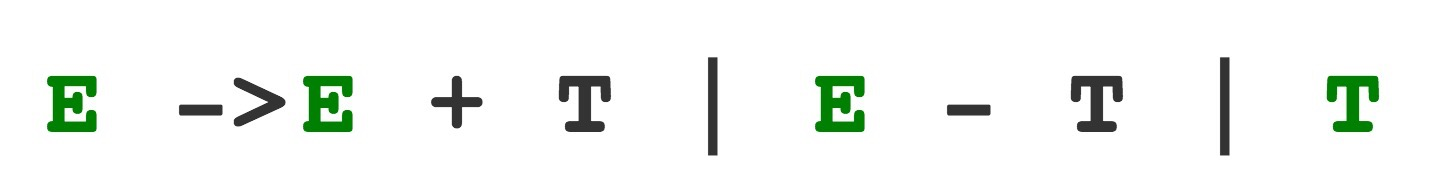
\includegraphics[width=0.7\linewidth]{img/recursive.jpg}
\caption{左递归消除,图中标记出将会改变的元素}
\label{fig:recursive.jpg}
\end{figure}
\subsection{具体的动画的例子}
动画中有纯粹展示类型的动画,比如其中的一个左递归消除的动画,它实现了按
步骤完成的整体动画,也提供了可以供用户单步进行的动画,用户也能够回退已
经执行过的动画,这些都在系统中实现了,但是,用户不能再动画运行过程中干
预动画的内容,也就是,它是一个纯粹的动画,甚至我们实现中就是将这个动画
对应的算法执行完毕之后,才开始进行动画,也就是说,动画的步骤是被实现记
录好了。
然而,系统中,并不只有这种类型的动画,另外也设计了一种动画,这种动画实
际上能够让用户参与进来,也就是说,用户可以改变某些变量,从而得到一个完
全不一样的动画形态,换句话说,用户不止可以在一开始的时候指定状态,甚至
可以在动画进行的过程中指定状态,从而让动画往不一样的方向发展。
根据动画的形态来区分系统中存在的动画,有这几种,分别是,形象化表达的动
画,比如消除左递归中,分别出现原本的产生式,接着,产生式的一部分被移除
画面,另一部分保留在画面中,并且缩进成一个紧凑的形态,这之后,,这个紧
凑的形态,再次伸展开来,插入新的字符,从而得到了产生式A,而此后,这个
产生式A再次消失。这个动画结束以后,再浮现出新的一组产生式,这组产生式
的字符就由刚才最先被移除的那部分字符组成,然后,再附上新的字符,使得产
生式消除左递归的过程得到充分地展现。
\subsection{动画背后的道理}
要理解这些动画是如何设计出来的,那么需要先理解状态机是如何工作的,我们
在设计动画的时候,是把动画的表现抽离出来的,也就是,并不是将动画放入我
们所编写的算法中,而是作为独立的模块存在的,它算法本身的实现,几乎没有
什么联系,除了算法本身的特点将影响我们所采用的动画这一点以外。算法本身
运行的时候,自身是一个状态机,也就是,它从一个状态进入到另一个状态,或
者也可以回去,等等,并不与外界产生交互。然而,我们在外界是可以控制算法
是如何运行的。而之后,我们提取状态机,也就是算法,运行过程中,是如何改
变状态的,把这些状态的改变都记录下来,而最终就是根据这些状态的改变来生
成动画的。对于那种动画进行过程中,却可以改变算法的状态的,其实就是利用
了,状态机本身不对外界产生影响,但是,外界却能够对状态机产生影响这个道
理。而且,因为状态机记录的内容并不会丢失掉,不会因为算法重新执行到哪一
个而导致之前的步骤消失,所有的步骤都被完整记录下来。当外界去改变状态机
的一些状态走向的时候,也只是改变状态机未来的状态,也就是说,状态机还没
有走过的状态,所以不用担心状态丢失而不能有效表达动画。从这个层面上看,
这类型的动画,就不是离线的,而是实时的,围绕着用户的交互而进行的一种动
画。
除了状态机这样的观点来做动画以外,我其实更喜欢把算法看做是一系列的动作
制定器,在算法运行的时候,在程序的一些关键点中,加入算法记录函数,也就
是算法记录点,在这些算法记录点中,我可以提取动画所需要的数据,之后通过
获取这些算法记录点,我们可以将动画展示出来。当然,这样子实现的动画,是
没有额外的交互功能的,所谓额外交互功能就是除了单点执行中的前进后退,完
整执行一段动画这俩个主要的动能以外,没有别的交互功能。当然,如果暴露出
更多的信息,通过这些算法记录点,那么还可以让用户观测到这个算法执行到当
前时间段的时候,所有当前的变量信息、环境信息等等。这种方式,实际上就是
我们初次版本所要实现的方式,而更理想的状态机的方式,其实也是在这种方式
上面进行改造的结果。然而,在实现时,状态机的方式还有更多的问题需要解决,
所以在后续的开发中,我们要逐一解决这些问题。
\subsection{交互的要点}
动画交互需要注意分出来,哪一些是必要的部分,而哪一些是不必要的信息。还
有哪一些是要一直强调的部分,哪一些是在用户需要的时候才展现给用户看的部
分。具体来说的话,就是指的,在动画演示的过程中,有一些部分,要着重强调
出来,比如说,算法执行的主要步骤,算法在某一个时刻,实际上是对什么进行
操作,做了哪些操作,如果有办法,甚至还要体现为什么要做这些操作,让学生
可以通过看到这些动画,就能明白这些操作的含义,可以自己去完成这些操作。
除此之外,还有一些部分是在算法演示中不一定被强调的,比如当前执行的循环
次数,当前某个变量的值,这些东西的存在,可能会干扰学生进行感性的思考,
但是这些东西也必须存在,如果因为为了美观和可读性而直接牺牲了这些数据,
那么得到的内容是不完整的。当学生想要深入思考这些变量的变化的时候,就需
要这些更细节的内容,只是依靠图上的变化,是不足以让学生了解这些细节的变
化。
